% Author: Till Tantau
% Source: The PGF/TikZ manual
\documentclass{article}

\usepackage[latin1]{inputenc}
\usepackage{tikz}

% GNUPLOT required
\begin{document}
\pagestyle{empty}


\begin{tikzpicture}[domain=-1:7.5]
    \draw[very thin,color=gray] (-1.25,-1) grid (7.5,4);
    \draw[->] (-1.5,0) -- (8,0) node[right] {$t$};
    \draw[->] (0,-1.2) -- (0,4.2) node[above] {$x(t)$};
    \draw[color=red] plot[id=grafica1] function{0.667*(exp(-2*x) - exp(-x/2))} 
        node[above left] {$x(t) = \frac{2}{3}(e^{-2t} - e^{-\frac{t}{2}}) $};
        
    \foreach \x in {-1,1,3,5,7} \draw (\x cm,4pt) -- (\x cm,-4pt) node[anchor=north] {$\x$};    
    \foreach \helpy in {-0.5,1,3} \draw (4pt, \helpy cm) -- (-4pt, \helpy) node [anchor=east] {$\helpy$};
    
\end{tikzpicture}

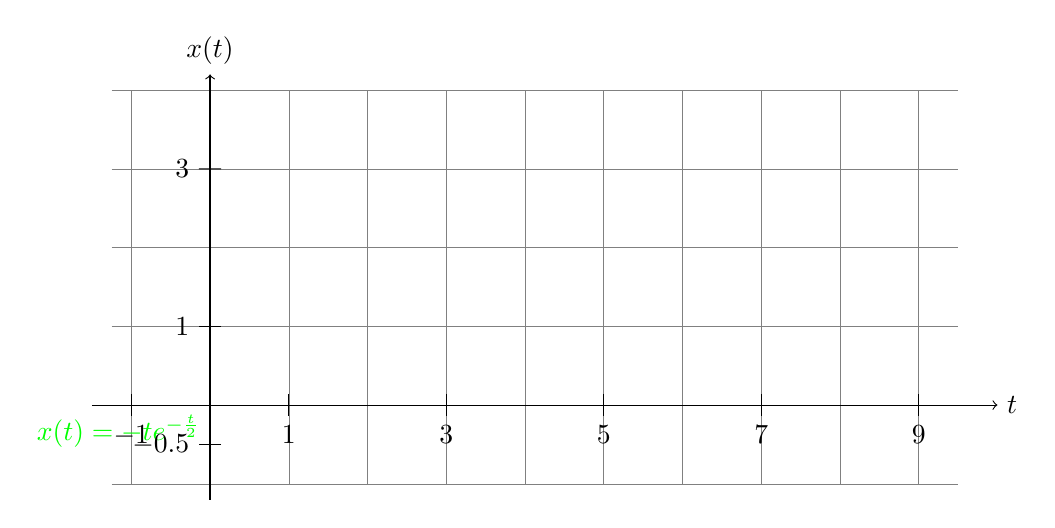
\begin{tikzpicture}[domain=-1.5:9]
    \draw[very thin,color=gray] (-1.25,-1) grid (9.5,4);
    \draw[->] (-1.5,0) -- (10,0) node[right] {$t$};
    \draw[->] (0,-1.2) -- (0,4.2) node[above] {$x(t)$};
    \draw[color=green] plot[id=grafica2] function{-x*exp(-x/2)} 
        node[below left] {$x(t) = -te^{-\frac{t}{2}} $};
        
    \foreach \x in {-1,1,3,5,7,9} \draw (\x cm,4pt) -- (\x cm,-4pt) node[anchor=north] {$\x$};    
    \foreach \helpy in {-0.5,1,3} \draw (4pt, \helpy cm) -- (-4pt, \helpy) node [anchor=east] {$\helpy$};
\end{tikzpicture}

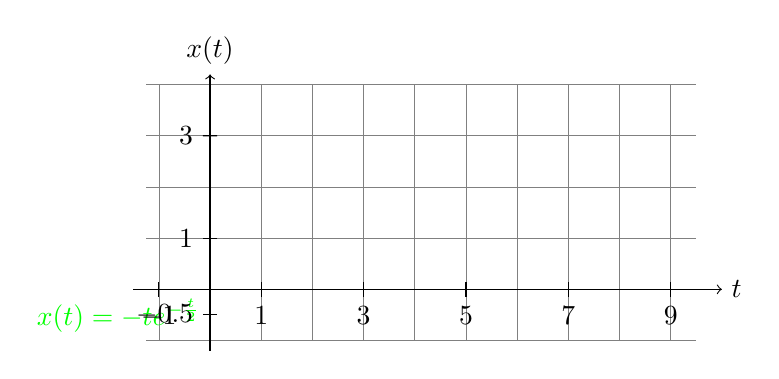
\begin{tikzpicture}[domain=--10:10,scale=0.65]
    \draw[very thin,color=gray] (-1.25,-1) grid (9.5,4);
    \draw[->] (-1.5,0) -- (10,0) node[right] {$t$};
    \draw[->] (0,-1.2) -- (0,4.2) node[above] {$x(t)$};
    \draw[color=green] plot[id=grafica3] function{-4*exp(-0.1*x)*sin(0.25*x)} 
        node[below left] {$x(t) = -te^{-\frac{t}{2}} $};
        
    \foreach \x in {-1,1,3,5,7,9} \draw (\x cm,4pt) -- (\x cm,-4pt) node[anchor=north] {$\x$};    
    \foreach \helpy in {-0.5,1,3} \draw (4pt, \helpy cm) -- (-4pt, \helpy) node [anchor=east] {$\helpy$};
\end{tikzpicture}

\end{document}
